\documentclass[12pt]{article}
\usepackage[margin=1in]{geometry}
\usepackage{setspace}
\usepackage[T1]{fontenc}
\usepackage{newtxtext,newtxmath}
\usepackage{graphicx}
\usepackage{float}
\usepackage{booktabs}
\usepackage{tabularx}
\usepackage{array}
\usepackage{ragged2e}
\usepackage{caption}
\usepackage[table]{xcolor}
\usepackage{tikz}
\usepackage{enumitem}
\usepackage{hyperref}
\usetikzlibrary{arrows.meta,positioning,fit,shapes.geometric}


%% ── Spacing / layout ──────────────────────────────────────────────────────────
\doublespacing
\setlength{\parindent}{0pt}
\setlength{\parskip}{0.55em}
\setlength{\tabcolsep}{6pt}
\renewcommand{\arraystretch}{1.25}
\setlength{\emergencystretch}{2em}


%% ── Stage palette (dark borders + light fills) ────────────────────────────────
\definecolor{stagecollect}{HTML}{365C8D}
\definecolor{stageclean}{HTML}{2E7D6E}
\definecolor{stageprep}{HTML}{C97A2B}
\definecolor{stagemine}{HTML}{7B4FA0}
\definecolor{lightcollect}{HTML}{EAF1F8}
\definecolor{lightclean}{HTML}{E8F4F1}
\definecolor{lightprep}{HTML}{FBF1E4}
\definecolor{lightmine}{HTML}{F1E9F8}

%% ── Within-table accent shades (deeper variants for "primary" rows) ───────────
%% These let primary and supporting rows differ within the same stage block.
\definecolor{deepcollect}{HTML}{D0E3F5}   % slightly darker collect shade
\definecolor{deepclean}{HTML}{C8EAE4}     % slightly darker clean shade
\definecolor{deepprep}{HTML}{F5E2C5}      % slightly darker prep shade
\definecolor{deepmine}{HTML}{E0D0F4}      % slightly darker mine shade -- primary contrasts
\definecolor{midmine}{HTML}{EBE0F8}       % mid shade -- supporting contrasts
\definecolor{palmine}{HTML}{F5F0FB}       % pale shade -- interaction / weakest contrasts

%% ── Shared chrome ─────────────────────────────────────────────────────────────
\definecolor{tableheader}{HTML}{F2F2F2}
\definecolor{gridgray}{HTML}{D9D9D9}

%% ── Sample-group swatches for the design table ───────────────────────────────
\definecolor{ipsiFF}{HTML}{D6EAF8}       % ipsi / FF
\definecolor{ipsiCRE}{HTML}{D5F5E3}      % ipsi / CRE
\definecolor{contraFF}{HTML}{FCF3CF}     % contra / FF
\definecolor{contraCRE}{HTML}{FADBD8}    % contra / CRE


%% ── Column types ──────────────────────────────────────────────────────────────
\newcolumntype{Y}{>{\RaggedRight\arraybackslash}X}
\newcolumntype{Z}{>{\centering\arraybackslash}X}


%% ── Stage label macro ────────────────────────────────────────────────────────
\newcommand{\stagelabel}[2]{\fcolorbox{#1}{#1!12}{\textcolor{#1}{\textbf{#2}}}}

%% ── Contrast priority labels ─────────────────────────────────────────────────
\newcommand{\primary}{\textcolor{stagemine}{\textbf{primary}}}
\newcommand{\supporting}{\textcolor{stagemine}{supporting}}
\newcommand{\contextual}{\textcolor{gray}{contextual}}


\title{Materials and Methods Draft\\Mouse DRG RNA-seq Follow-up Project}
\author{Piter Garcia}
\date{Draft prepared for BIOL550}


\begin{document}
\maketitle


\section{Materials and Methods}


This section describes the \texttt{mouse\_new} analysis workflow as a reproducible bioinformatics pipeline organized around four computational stages: \textbf{Data Collection}, \textbf{Data Cleaning}, \textbf{Data Preparation}, and \textbf{Data Mining and Interpretation}. That structure makes both the biological context and the computational handoffs explicit, from raw sequence acquisition through differential expression and enrichment analysis. Each stage is documented by a pipeline summary table and a matching figure; figures explain how each stage works, while tables capture the concrete inputs, tools, outputs, and key metrics produced. Color coding within each table reflects stage identity at the row level, with additional within-stage shading used in the Data Mining section to distinguish primary, supporting, and contextual contrasts from one another.


%% ── Overall pipeline figure ──────────────────────────────────────────────────
\begin{figure}[H]
\centering
\resizebox{\textwidth}{!}{%
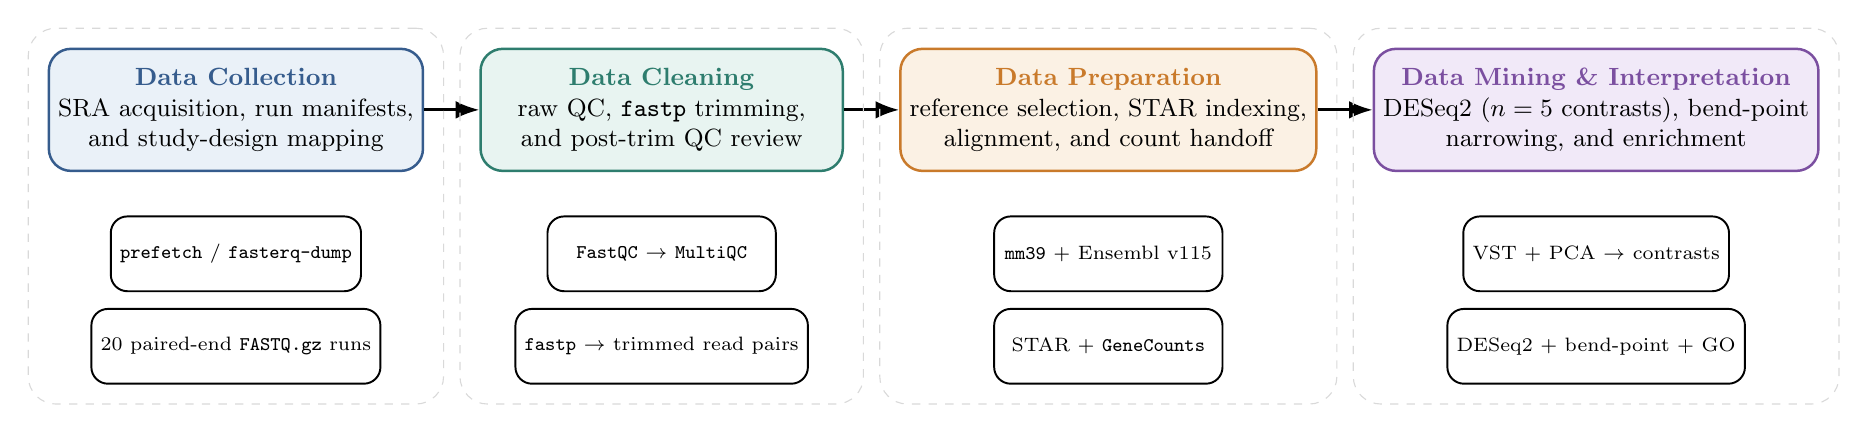
\begin{tikzpicture}[
  node distance=1.1cm and 0.7cm,
  stage/.style={draw, rounded corners=8pt, line width=0.9pt, minimum width=4.6cm,
                minimum height=1.55cm, align=center, font=\small},
  mini/.style={draw, rounded corners=6pt, line width=0.7pt, minimum width=2.9cm,
               minimum height=0.95cm, align=center, font=\scriptsize, fill=white},
  arrow/.style={-{Latex[length=3mm]}, line width=1pt}
]

\node[stage, fill=lightcollect, draw=stagecollect] (s1)
  {\textcolor{stagecollect}{\textbf{Data Collection}}\\
   SRA acquisition, run manifests,\\and study-design mapping};
\node[stage, fill=lightclean, draw=stageclean, right=of s1] (s2)
  {\textcolor{stageclean}{\textbf{Data Cleaning}}\\
   raw QC, \texttt{fastp} trimming,\\and post-trim QC review};
\node[stage, fill=lightprep, draw=stageprep, right=of s2] (s3)
  {\textcolor{stageprep}{\textbf{Data Preparation}}\\
   reference selection, STAR indexing,\\alignment, and count handoff};
\node[stage, fill=lightmine, draw=stagemine, right=of s3] (s4)
  {\textcolor{stagemine}{\textbf{Data Mining \& Interpretation}}\\
   DESeq2 ($n=5$ contrasts), bend-point\\narrowing, and enrichment};

\draw[arrow] (s1) -- (s2);
\draw[arrow] (s2) -- (s3);
\draw[arrow] (s3) -- (s4);

\node[mini, below=0.55cm of s1] (s1a) {\texttt{prefetch} / \texttt{fasterq-dump}};
\node[mini, below=0.55cm of s2] (s2a) {\texttt{FastQC} $\rightarrow$ \texttt{MultiQC}};
\node[mini, below=0.55cm of s3] (s3a) {\texttt{mm39} + Ensembl v115};
\node[mini, below=0.55cm of s4] (s4a) {VST + PCA $\rightarrow$ contrasts};

\node[mini, below=0.2cm of s1a] (s1b) {20 paired-end \texttt{FASTQ.gz} runs};
\node[mini, below=0.2cm of s2a] (s2b) {\texttt{fastp} $\rightarrow$ trimmed read pairs};
\node[mini, below=0.2cm of s3a] (s3b) {STAR + \texttt{GeneCounts}};
\node[mini, below=0.2cm of s4a] (s4b) {DESeq2 + bend-point + GO};

\node[draw=gridgray, dashed, rounded corners=10pt,
      fit=(s1)(s1a)(s1b), inner sep=7pt] {};
\node[draw=gridgray, dashed, rounded corners=10pt,
      fit=(s2)(s2a)(s2b), inner sep=7pt] {};
\node[draw=gridgray, dashed, rounded corners=10pt,
      fit=(s3)(s3a)(s3b), inner sep=7pt] {};
\node[draw=gridgray, dashed, rounded corners=10pt,
      fit=(s4)(s4a)(s4b), inner sep=7pt] {};
\end{tikzpicture}%
}
\caption{End-to-end structure of the \texttt{mouse\_new} RNA-seq workflow organized into four
  reproducible computational stages.  The Data Mining stage encompasses five DESeq2 contrasts
  (two primary side-specific, two genotype-focused, one interaction); the primary side-specific
  contrasts are \texttt{ipsi\_vs\_contra\_in\_ff} and \texttt{ipsi\_vs\_contra\_in\_cre}.}
\label{fig:overall_pipeline}
\end{figure}


%% ═══════════════════════════════════════════════════════════════════════════════
\subsection{Data Collection: SRA Acquisition and Sample Organization}

The study analyzed the mouse dorsal root ganglion (DRG) bulk RNA-seq dataset associated with
\texttt{SRP618841} (BioProject \texttt{PRJNA1017789}; GEO \texttt{GSE243308}).
Sequence runs were obtained from the NCBI Sequence Read Archive using local acquisition wrappers
around \texttt{prefetch} and \texttt{fasterq-dump}, and the paired-end outputs were stored as
compressed \texttt{FASTQ.gz} files so the same inputs could be reused across QC, alignment, and
notebook-based downstream analysis without modification.
The working subset consisted of 20 DRG samples generated on a NovaSeq X platform under a spinal
cord injury (SCI) design, all sampled at 1 day post-injury (1~dpi).

Sample metadata were structured as a design table rather than as loose file names, with each run
labeled by side class (\texttt{ipsi} or \texttt{contra}) and genotype class (\texttt{ff} or
\texttt{cre}).
The 20 samples split into four balanced groups of five replicates each:
\texttt{ipsi\_ff}, \texttt{ipsi\_cre}, \texttt{contra\_ff}, and \texttt{contra\_cre},
all belonging to the family \texttt{family\_drg\_novaseqx}.
Table~\ref{tab:design_table} shows the full per-sample design used in all downstream contrasts.
Making the biological groupings explicit before any exploratory or inferential analysis was a
deliberate design choice: sample structure had to be confirmed before gene-level and
pathway-level claims could be trusted.


%% ── Design table ─────────────────────────────────────────────────────────────
\begin{table}[H]
\centering
\small
\caption{Per-sample design table for the \texttt{family\_drg\_novaseqx} subset
  ($n = 20$). Color shading encodes the four condition groups used in all DESeq2 contrasts.
  All samples: tissue = DRG, treatment = Spinal Cord Injury 1\,dpi, platform = NovaSeq X,
  post-\texttt{fastp} GC status = WARN (monitored; alignment metrics confirmed no downstream
  penalty; see Section~\ref{sec:cleaning}).}
\label{tab:design_table}
\begin{tabularx}{\textwidth}{l l >{\centering\arraybackslash}p{1.6cm}
                              >{\centering\arraybackslash}p{1.6cm}
                              >{\centering\arraybackslash}p{2.2cm} Y}
\toprule
\rowcolor{tableheader}
\textbf{SRR} & \textbf{Replicate} & \textbf{Side} & \textbf{Geno} &
\textbf{Condition group} & \textbf{Genotype label} \\
\midrule
\rowcolor{ipsiFF}
SRR35329978 & H65  & ipsi  & ff  & ipsi\_ff  & Wildtype \\
\rowcolor{ipsiFF}
SRR35329984 & H62  & ipsi  & ff  & ipsi\_ff  & Wildtype \\
\rowcolor{ipsiFF}
SRR35329986 & H63  & ipsi  & ff  & ipsi\_ff  & Wildtype \\
\rowcolor{ipsiFF}
SRR35329991 & H96  & ipsi  & ff  & ipsi\_ff  & Wildtype \\
\rowcolor{ipsiFF}
SRR35329992 & H97  & ipsi  & ff  & ipsi\_ff  & Wildtype \\
\midrule
\rowcolor{ipsiCRE}
SRR35329977 & H64  & ipsi  & cre & ipsi\_cre & CRE \\
\rowcolor{ipsiCRE}
SRR35329983 & H61  & ipsi  & cre & ipsi\_cre & CRE \\
\rowcolor{ipsiCRE}
SRR35329987 & H95  & ipsi  & cre & ipsi\_cre & CRE \\
\rowcolor{ipsiCRE}
SRR35329993 & H99  & ipsi  & cre & ipsi\_cre & CRE \\
\rowcolor{ipsiCRE}
SRR35329994 & H100 & ipsi  & cre & ipsi\_cre & CRE \\
\midrule
\rowcolor{contraFF}
SRR35329979 & H96  & contra & ff  & contra\_ff & Wildtype \\
\rowcolor{contraFF}
SRR35329980 & H97  & contra & ff  & contra\_ff & Wildtype \\
\rowcolor{contraFF}
SRR35329981 & H65  & contra & ff  & contra\_ff & Wildtype \\
\rowcolor{contraFF}
SRR35329982 & H62  & contra & ff  & contra\_ff & Wildtype \\
\rowcolor{contraFF}
SRR35329989 & H63  & contra & ff  & contra\_ff & Wildtype \\
\midrule
\rowcolor{contraCRE}
SRR35329985 & H64  & contra & cre & contra\_cre & CRE \\
\rowcolor{contraCRE}
SRR35329988 & H99  & contra & cre & contra\_cre & CRE \\
\rowcolor{contraCRE}
SRR35329990 & H100 & contra & cre & contra\_cre & CRE \\
\rowcolor{contraCRE}
SRR35329995 & H95  & contra & cre & contra\_cre & CRE \\
\rowcolor{contraCRE}
SRR35329996 & H6   & contra & cre & contra\_cre & CRE \\
\bottomrule
\multicolumn{6}{l}{\small
  \colorbox{ipsiFF}{\phantom{X}}~ipsi / FF \quad
  \colorbox{ipsiCRE}{\phantom{X}}~ipsi / CRE \quad
  \colorbox{contraFF}{\phantom{X}}~contra / FF \quad
  \colorbox{contraCRE}{\phantom{X}}~contra / CRE}
\end{tabularx}
\end{table}


%% ── Stage summary table ───────────────────────────────────────────────────────
\begin{table}[H]
\centering
\small
\caption{Data Collection stage summary.}
\label{tab:data_collection}
\begin{tabularx}{\textwidth}{>{\columncolor{tableheader}}p{2.25cm} Y Y Y Y}
\toprule
\textbf{Input} & \textbf{Tool or source} & \textbf{Output} &
\textbf{Purpose} & \textbf{Key stage metrics or artifacts} \\
\midrule
\rowcolor{lightcollect}
Public study accession (\texttt{SRP618841}) &
SRA Toolkit and local acquisition wrappers &
20 paired-end \texttt{FASTQ.gz} runs and run manifest &
Reconstruct the working DRG subset locally from public data &
BioProject \texttt{PRJNA1017789}; GEO \texttt{GSE243308};
all 20 samples retained in the active DRG subset \\
\rowcolor{deepcollect}
Run metadata and sample annotations &
Project design table assembly &
Structured per-sample manifest (Table~\ref{tab:design_table})
used by all downstream scripts and notebooks &
Preserve the biological labels (\texttt{side\_class},
\texttt{geno\_class}) attached to each sequencing run &
10 ipsi (5 ff + 5 cre), 10 contra (5 ff + 5 cre);
family = \texttt{family\_drg\_novaseqx};
design formula =
\texttt{\textasciitilde{} side\_class + geno\_class + side\_class:geno\_class} \\
\bottomrule
\end{tabularx}
\end{table}


\begin{figure}[H]
\centering

\includegraphics[width=\textwidth]{assets_methods/data_collection_stage.png}
\caption{Data Collection stage summary figure. The panel shows the public accession lineage
  (\texttt{SRP618841} / \texttt{PRJNA1017789} / \texttt{GSE243308}), the local acquisition
  handoff via \texttt{prefetch} and \texttt{fasterq-dump}, and the four balanced subgroups
  (\texttt{ipsi\_ff}, \texttt{ipsi\_cre}, \texttt{contra\_ff}, \texttt{contra\_cre})
  that define all downstream contrasts.}
\label{fig:data_collection}
\end{figure}


%% ═══════════════════════════════════════════════════════════════════════════════
\subsection{Data Cleaning: Quality Control and Read Trimming}
\label{sec:cleaning}

Raw sequence quality was assessed with \texttt{FastQC}, and consolidated summaries were reviewed
with \texttt{MultiQC} to evaluate adapter contamination, sequence-content anomalies,
read-length behavior, and per-sample warning patterns across all 40 raw read files
(20 samples, two mates each).
\texttt{fastp} v0.23.2 was retained as the canonical trimming step following earlier remediation
work on the mouse project; it resolved adapter-related signal more effectively than the earlier
FASTX-based baseline while preserving a fully reproducible paired-end workflow.
The trimming configuration applied paired-end adapter detection (\texttt{--detect\_adapter\_for\_pe}),
tail trimming (\texttt{--cut\_tail}), a mean-quality cutoff of 20, a minimum retained length of
30 bases, poly-G trimming, and per-sample HTML/JSON reporting.

Post-trimming \texttt{FastQC} runs confirmed that \texttt{Adapter Content} improved from 40/40
raw-file failures to 80/80 post-trim passes.
One pattern persisted after trimming and required explicit documentation: all 20 DRG samples
carried a \texttt{Per Sequence GC Content} WARN flag in the corrected trimmed-only shared
MultiQC report.
The GC WARN subset did not map to a single biological condition (it was not confined to
injury vs.\ control, nor to FF vs.\ CRE), which made targeted removal unjustified at this
stage (see also Section~\ref{sec:preparation}).
The working decision, documented in the project remediation notes, was to treat the GC WARN
status as a monitored flag, proceed to alignment, and use per-sample STAR metrics to determine
whether the WARN samples showed any downstream penalty relative to a hypothetical PASS cohort.
As confirmed in the alignment summary (Section~\ref{sec:preparation}), the lowest uniquely
mapped rate in the cohort was 92.50\%, with the cohort median at 93.24\%, so the GC WARN
pattern did not translate into a meaningful alignment quality penalty.


\begin{table}[H]
\centering
\small
\caption{Data Cleaning stage summary. Three sub-steps are shown: raw QC baseline,
  \texttt{fastp} trimming, and post-trim QC verification. The two MultiQC runs correspond
  to the corrected stage-specific reports (raw-only and trimmed-only), not the earlier
  mixed comparison report that was superseded.}
\label{tab:data_cleaning}
\begin{tabularx}{\textwidth}{>{\columncolor{tableheader}}p{2.25cm} Y Y Y Y}
\toprule
\textbf{Input} & \textbf{Tool or source} & \textbf{Output} &
\textbf{Purpose} & \textbf{Key stage metrics or artifacts} \\
\midrule
\rowcolor{lightclean}
Raw paired-end \texttt{FASTQ.gz} files (20 samples, 40 read files) &
\texttt{FastQC} + \texttt{MultiQC} (raw-only report) &
Raw QC bundle; module-level warning table &
Establish baseline sequencing quality before cleanup &
\texttt{Adapter Content}: 40/40 raw files \textbf{FAIL};
\texttt{Per Sequence GC Content}: pattern noted;
raw-only MultiQC retained as authoritative pre-trim reference \\
\rowcolor{deepclean}
Raw paired-end reads + QC feedback &
\texttt{fastp} v0.23.2 &
Trimmed paired-end reads; per-sample HTML/JSON reports &
Remove adapter-related and low-quality trailing sequence while preserving paired reads &
Adapter detection (\texttt{--detect\_adapter\_for\_pe}),
tail trim (\texttt{--cut\_tail}), mean-Q cutoff 20,
min-length 30, poly-G trim;
20 samples $\times$ 2 mate files trimmed \\
\rowcolor{lightclean}
Trimmed read pairs &
\texttt{FastQC} + \texttt{MultiQC} (trimmed-only report) &
Post-trim QC bundle; before/after module comparison &
Verify that cleanup improved the read set before alignment &
\texttt{Adapter Content}: 40/40 fail $\rightarrow$ 80/80 pass;
\texttt{Per Sequence GC Content}: 0 FAIL, all 20 samples = WARN
(monitored; GC WARN subset does not correspond to one biological condition;
alignment metrics evaluated in Section~\ref{sec:preparation}) \\
\bottomrule
\end{tabularx}
\end{table}


\begin{figure}[H]
\centering

\includegraphics[width=\textwidth]{assets_methods/data_cleaning_stage.png}
\caption{Data Cleaning stage artifacts from the stage-specific QC review.
  Panel~(a): module-level FastQC transition from raw to trimmed reads showing the
  \texttt{Adapter Content} improvement from 40/40 fail to 80/80 pass and the residual
  GC WARN pattern.
  Panel~(b): MultiQC general-statistics summary (trimmed-only report) used to confirm
  per-cohort preprocessing behavior; the two authoritative stage-specific reports
  (raw-only and trimmed-only) are retained as separate artifacts.}
\label{fig:data_cleaning}
\end{figure}


%% ═══════════════════════════════════════════════════════════════════════════════
\subsection{Data Preparation: Reference Selection and Alignment}
\label{sec:preparation}

The cleaned reads were aligned against the \textit{Mus musculus} \texttt{GRCm39} primary
assembly (\texttt{Mus\_musculus.GRCm39.dna.primary\_assembly.fa}) with the matching Ensembl
release~115 annotation (\texttt{Mus\_musculus.GRCm39.115.gtf}).
A STAR genome index was built with \texttt{sjdbOverhang}~= 150 to match the 151-bp paired-end
read length of the NovaSeq X runs in the DRG subset.
Alignment was performed with STAR using gzip-aware input reading, coordinate-sorted BAM output,
and \texttt{GeneCounts} quantification, so the same alignment step produced both the sorted BAM
and the count-ready gene summary for each sample.

Each sample produced three output files used in downstream analysis: a sorted BAM, a
\texttt{Log.final.out} alignment report, and a \texttt{ReadsPerGene.out.tab} count table.
The per-sample STAR metrics were aggregated into a cohort-level alignment summary
(Table~\ref{tab:data_preparation}), which served as the explicit quality checkpoint before
differential expression modeling.
Across all 20 NovaSeq X DRG samples, the median unique mapping rate was 93.24\% and the median
multi-mapping rate was 5.10\%; the five lowest individual unique-mapping rates were
92.50\%, 92.67\%, 92.70\%, 92.74\%, and 93.08\%, confirming that the GC WARN cohort
(Section~\ref{sec:cleaning}) did not carry a meaningful alignment penalty.
Reverse-stranded assignment burden remained low across the cohort
(median \texttt{noFeature} $\approx$3.82\%; median \texttt{ambiguous} $\approx$1.77\%),
consistent with the expected behavior for a well-annotated mouse primary assembly.
The per-sample count outputs were then merged into a family-level gene-by-sample count matrix
using local merging scripts.


\begin{table}[H]
\centering
\small
\caption{Data Preparation stage summary. Three sub-steps are shown: reference and index
  preparation, alignment and per-sample output generation, and count-matrix assembly.
  All metrics are derived from the saved \texttt{mouse\_alignment\_sample\_summary.tsv} and
  the per-GC-status and per-platform median tables.}
\label{tab:data_preparation}
\begin{tabularx}{\textwidth}{>{\columncolor{tableheader}}p{2.25cm} Y Y Y Y}
\toprule
\textbf{Input} & \textbf{Tool or source} & \textbf{Output} &
\textbf{Purpose} & \textbf{Key stage metrics or artifacts} \\
\midrule
\rowcolor{lightprep}
Trimmed paired-end reads &
Ensembl mouse primary assembly + GTF &
Reference FASTA/GTF pair and STAR genome index &
Build a coordinate system matched to the current mouse annotation &
\texttt{GRCm39} primary assembly; Ensembl v115;
\texttt{sjdbOverhang}~= 150 (matched to 151-bp read length) \\
\rowcolor{deepprep}
Trimmed reads + STAR index &
STAR with \texttt{--quantMode GeneCounts} &
Sorted BAMs, \texttt{Log.final.out}, and
\texttt{ReadsPerGene.out.tab} per sample &
Generate alignment and count outputs in one reproducible step;
evaluate mapping quality before differential expression &
Cohort median (NovaSeq X, $n=20$):
unique mapping = 93.24\%;
multi-mapping = 5.10\%;
lowest individual unique mapping = 92.50\%
(SRR35329995; CRE / contra);
GC-WARN cohort alignment metrics indistinguishable from
GC-PASS reference range \\
\rowcolor{lightprep}
Per-sample count outputs &
Local merging scripts and notebooks &
Family-level gene-by-sample count matrix;
cohort alignment summary table &
Convert per-sample outputs into a matrix suitable for
DESeq2 modeling &
Reverse-stranded assignment burden:
median \texttt{noFeature} $\approx$3.82\%;
median \texttt{ambiguous} $\approx$1.77\%;
final count matrix passed to DESeq2 \\
\bottomrule
\end{tabularx}
\end{table}


\begin{figure}[H]
\centering

\includegraphics[width=\textwidth]{assets_methods/data_preparation_stage.png}
\caption{Data Preparation stage artifacts from the saved STAR alignment outputs.
  Panel~(a): unique mapping rates by sample and by platform, with the five lowest-mapped
  samples annotated (range 92.50–93.08\%; all NovaSeq X / GC WARN, consistent with the
  rest of the cohort).
  Panel~(b): reverse-stranded assignment burden showing \texttt{noFeature} and
  \texttt{ambiguous} fractions by platform and GC status; low burden confirms appropriate
  strandedness settings and well-matched annotation.}
\label{fig:data_preparation}
\end{figure}


%% ═══════════════════════════════════════════════════════════════════════════════
\subsection{Data Mining and Interpretation: Differential Expression and Functional Analysis}

The STAR count outputs were merged into a gene-by-sample count matrix for the
\texttt{family\_drg\_novaseqx} subset and modeled with \texttt{DESeq2}.
Before modeling, genes with insufficient support across the family were filtered out,
reducing the tested set from 78{,}334 genes to 21{,}481 genes while retaining all 20 samples.
The full interaction model applied was:
\[ \texttt{\textasciitilde{}\ side\_class + geno\_class + side\_class{:}geno\_class} \]
which estimates both main effects and the genotype-by-side interaction term in a single model,
making all five contrasts extractable from the same fitted object without refitting.

The first interpretive checkpoint after fitting was principal component analysis (PCA) on the
variance-stabilized count matrix (VST).
The PCA confirmed that \texttt{side\_class} (ipsilateral vs.\ contralateral) drives the
dominant variance axis in the DRG cohort, with ipsi and contra samples separating clearly on
PC1.
Genotype effects were visible as secondary structure: within the ipsilateral group, FF/CRE
pairs showed PCA distances as small as~0.27 (SRR35329986/SRR35329987), while across the
contralateral group the maximum FF/CRE pair distance was~32.9
(SRR35329982/SRR35329990), reflecting a broader genotype-dependent variance component on the
contra side.
This PCA interpretation was locked before gene-level claims were made.

Five contrasts were extracted from the DESeq2 model and are summarized in
Table~\ref{tab:data_mining}.
The two primary side-specific contrasts---\texttt{ipsi\_vs\_contra\_in\_ff} and
\texttt{ipsi\_vs\_contra\_in\_cre}---produced the largest significant gene sets (7{,}023 and
7{,}541 genes at $\text{p}_{\text{adj}} < 0.05$, respectively) and are the central analytical
results of the paper.
The two genotype-focused contrasts (\texttt{geno\_in\_contra} and \texttt{geno\_in\_ipsi}) and
the interaction contrast are retained as supporting and contextual results.

Because the primary side-specific contrasts yielded very large significant-gene sets unsuitable
for direct follow-up, the workflow applied a custom bend-point rule based on ranked
\textit{p}-value distributions to derive a smaller, data-driven gene subset from each contrast.
The bend-point threshold for \texttt{ipsi\_vs\_contra\_in\_ff} was $1.37 \times 10^{-17}$,
yielding 709 selected genes from 7{,}023 significant; for \texttt{ipsi\_vs\_contra\_in\_cre}
the threshold was $8.40 \times 10^{-17}$, yielding 870 from 7{,}541.
Functional enrichment was then run on the bend-point-selected gene sets using \texttt{g:Profiler}
with GO Biological Process, KEGG, and Reactome sources.
For the main \texttt{ff} side-specific contrast, the retained enrichment outputs included
359~GO:BP terms, 18~KEGG terms, and 3~Reactome terms.
MA plots, volcano plots, and heatmaps were generated as downstream analytical products for all
five contrasts and are reserved for the Results section.


\begin{table}[H]
\centering
\small
\caption{Data Mining and Interpretation stage summary. Rows are ordered by contrast priority
  (primary $\rightarrow$ supporting $\rightarrow$ contextual) and shaded accordingly.
  Bend-point thresholds and selected gene counts are derived directly from the saved
  per-contrast \texttt{bendpoint\_summary.tsv} files.}
\label{tab:data_mining}
\begin{tabularx}{\textwidth}{>{\columncolor{tableheader}}p{2.0cm} Y Y Y Y}
\toprule
\textbf{Step / contrast} & \textbf{Tool or source} & \textbf{Output} &
\textbf{Purpose} & \textbf{Key metrics or artifacts} \\
\midrule

%% -- Modeling row
\rowcolor{lightmine}
\multicolumn{5}{l}{\textcolor{stagemine}{\textbf{Modeling and sample-structure check}}} \\
\rowcolor{lightmine}
Family count matrix + design table &
\texttt{DESeq2} &
Normalized counts, VST matrix, and fitted model object &
Model expression differences under the full interaction design;
confirm sample structure via PCA before gene-level claims &
20 samples retained;
genes filtered 78{,}334 $\rightarrow$ 21{,}481;
VST PCA: PC1 separates \texttt{side\_class};
minimum FF/CRE PCA pair distance = 0.27 (ipsi group);
maximum = 32.9 (contra group) \\
\addlinespace[0.3em]

%% -- Primary contrasts header
\rowcolor{deepmine}
\multicolumn{5}{l}{\textcolor{stagemine}{\textbf{Primary side-specific contrasts}
  (\primary)}} \\

%% -- ipsi_vs_contra_in_ff
\rowcolor{deepmine}
\texttt{ipsi\_vs\_ contra\_in\_ff} &
DESeq2 coef \texttt{side\_class\_ ipsi\_vs\_contra}; bend-point narrowing; \texttt{g:Profiler} &
Ordered \textit{p}-value table; bend-point gene set; GO/KEGG/Reactome enrichment table and plots &
Capture the injury-side DRG expression signal in the FF (wildtype) background &
21{,}466 genes tested;
7{,}023 significant ($p_{\text{adj}} < 0.05$);
bend-point threshold $= 1.37 \times 10^{-17}$;
709 selected;
enrichment: 359~GO:BP, 18~KEGG, 3~Reactome \\
\rowcolor{deepmine}

%% -- ipsi_vs_contra_in_cre
\texttt{ipsi\_vs\_ contra\_in\_cre} &
DESeq2 list \texttt{side\_class\_ipsi\_vs\_contra} + interaction term; bend-point narrowing; \texttt{g:Profiler} &
Ordered \textit{p}-value table; bend-point gene set; enrichment table and plots &
Capture the injury-side DRG expression signal in the CRE background;
compare signal breadth and pathway overlap with the FF contrast &
21{,}466 genes tested;
7{,}541 significant;
bend-point threshold $= 8.40 \times 10^{-17}$;
870 selected \\
\addlinespace[0.3em]

%% -- Supporting contrasts header
\rowcolor{midmine}
\multicolumn{5}{l}{\textcolor{stagemine}{\textbf{Genotype-focused contrasts}
  (\supporting)}} \\

%% -- geno_in_contra
\rowcolor{midmine}
\texttt{geno\_in\_ contra} &
DESeq2 coef \texttt{geno\_class\_ cre\_vs\_ff}; bend-point narrowing; \texttt{g:Profiler} &
Ordered \textit{p}-value table; bend-point gene set; enrichment table and plots &
Assess genotype-driven expression differences in contralateral DRG (uninjured reference side) &
21{,}466 genes tested;
891 significant;
bend-point threshold $= 2.13 \times 10^{-4}$;
267 selected \\
\rowcolor{midmine}
\texttt{geno\_in\_ ipsi} &
DESeq2 list (\texttt{geno\_class} + interaction term); bend-point narrowing &
Ordered \textit{p}-value table; bend-point gene set &
Assess genotype-driven differences on the injured ipsilateral side &
21{,}466 genes tested;
2 significant ($p_{\text{adj}} < 0.05$);
bend-point threshold $= 0.0143$;
113 selected below threshold \\
\addlinespace[0.3em]

%% -- Contextual contrast header
\rowcolor{palmine}
\multicolumn{5}{l}{\textcolor{gray}{\textbf{Interaction contrast}
  (\contextual)}} \\

%% -- interaction
\rowcolor{palmine}
\texttt{interaction} &
DESeq2 coef \texttt{side\_class\_ ipsi.geno\_class\_ cre}; bend-point narrowing &
Ordered \textit{p}-value table; bend-point gene set &
Identify genes whose ipsilateral vs.\ contralateral difference is specifically larger or smaller in CRE animals &
21{,}466 genes tested;
14 significant;
bend-point threshold $= 0.046$;
1{,}823 selected below a permissive bend-point \\
\bottomrule
\multicolumn{5}{l}{\small
  \colorbox{deepmine}{\phantom{X}}~Primary \quad
  \colorbox{midmine}{\phantom{X}}~Supporting \quad
  \colorbox{palmine}{\phantom{X}}~Contextual}
\end{tabularx}
\end{table}


\begin{figure}[H]
\centering
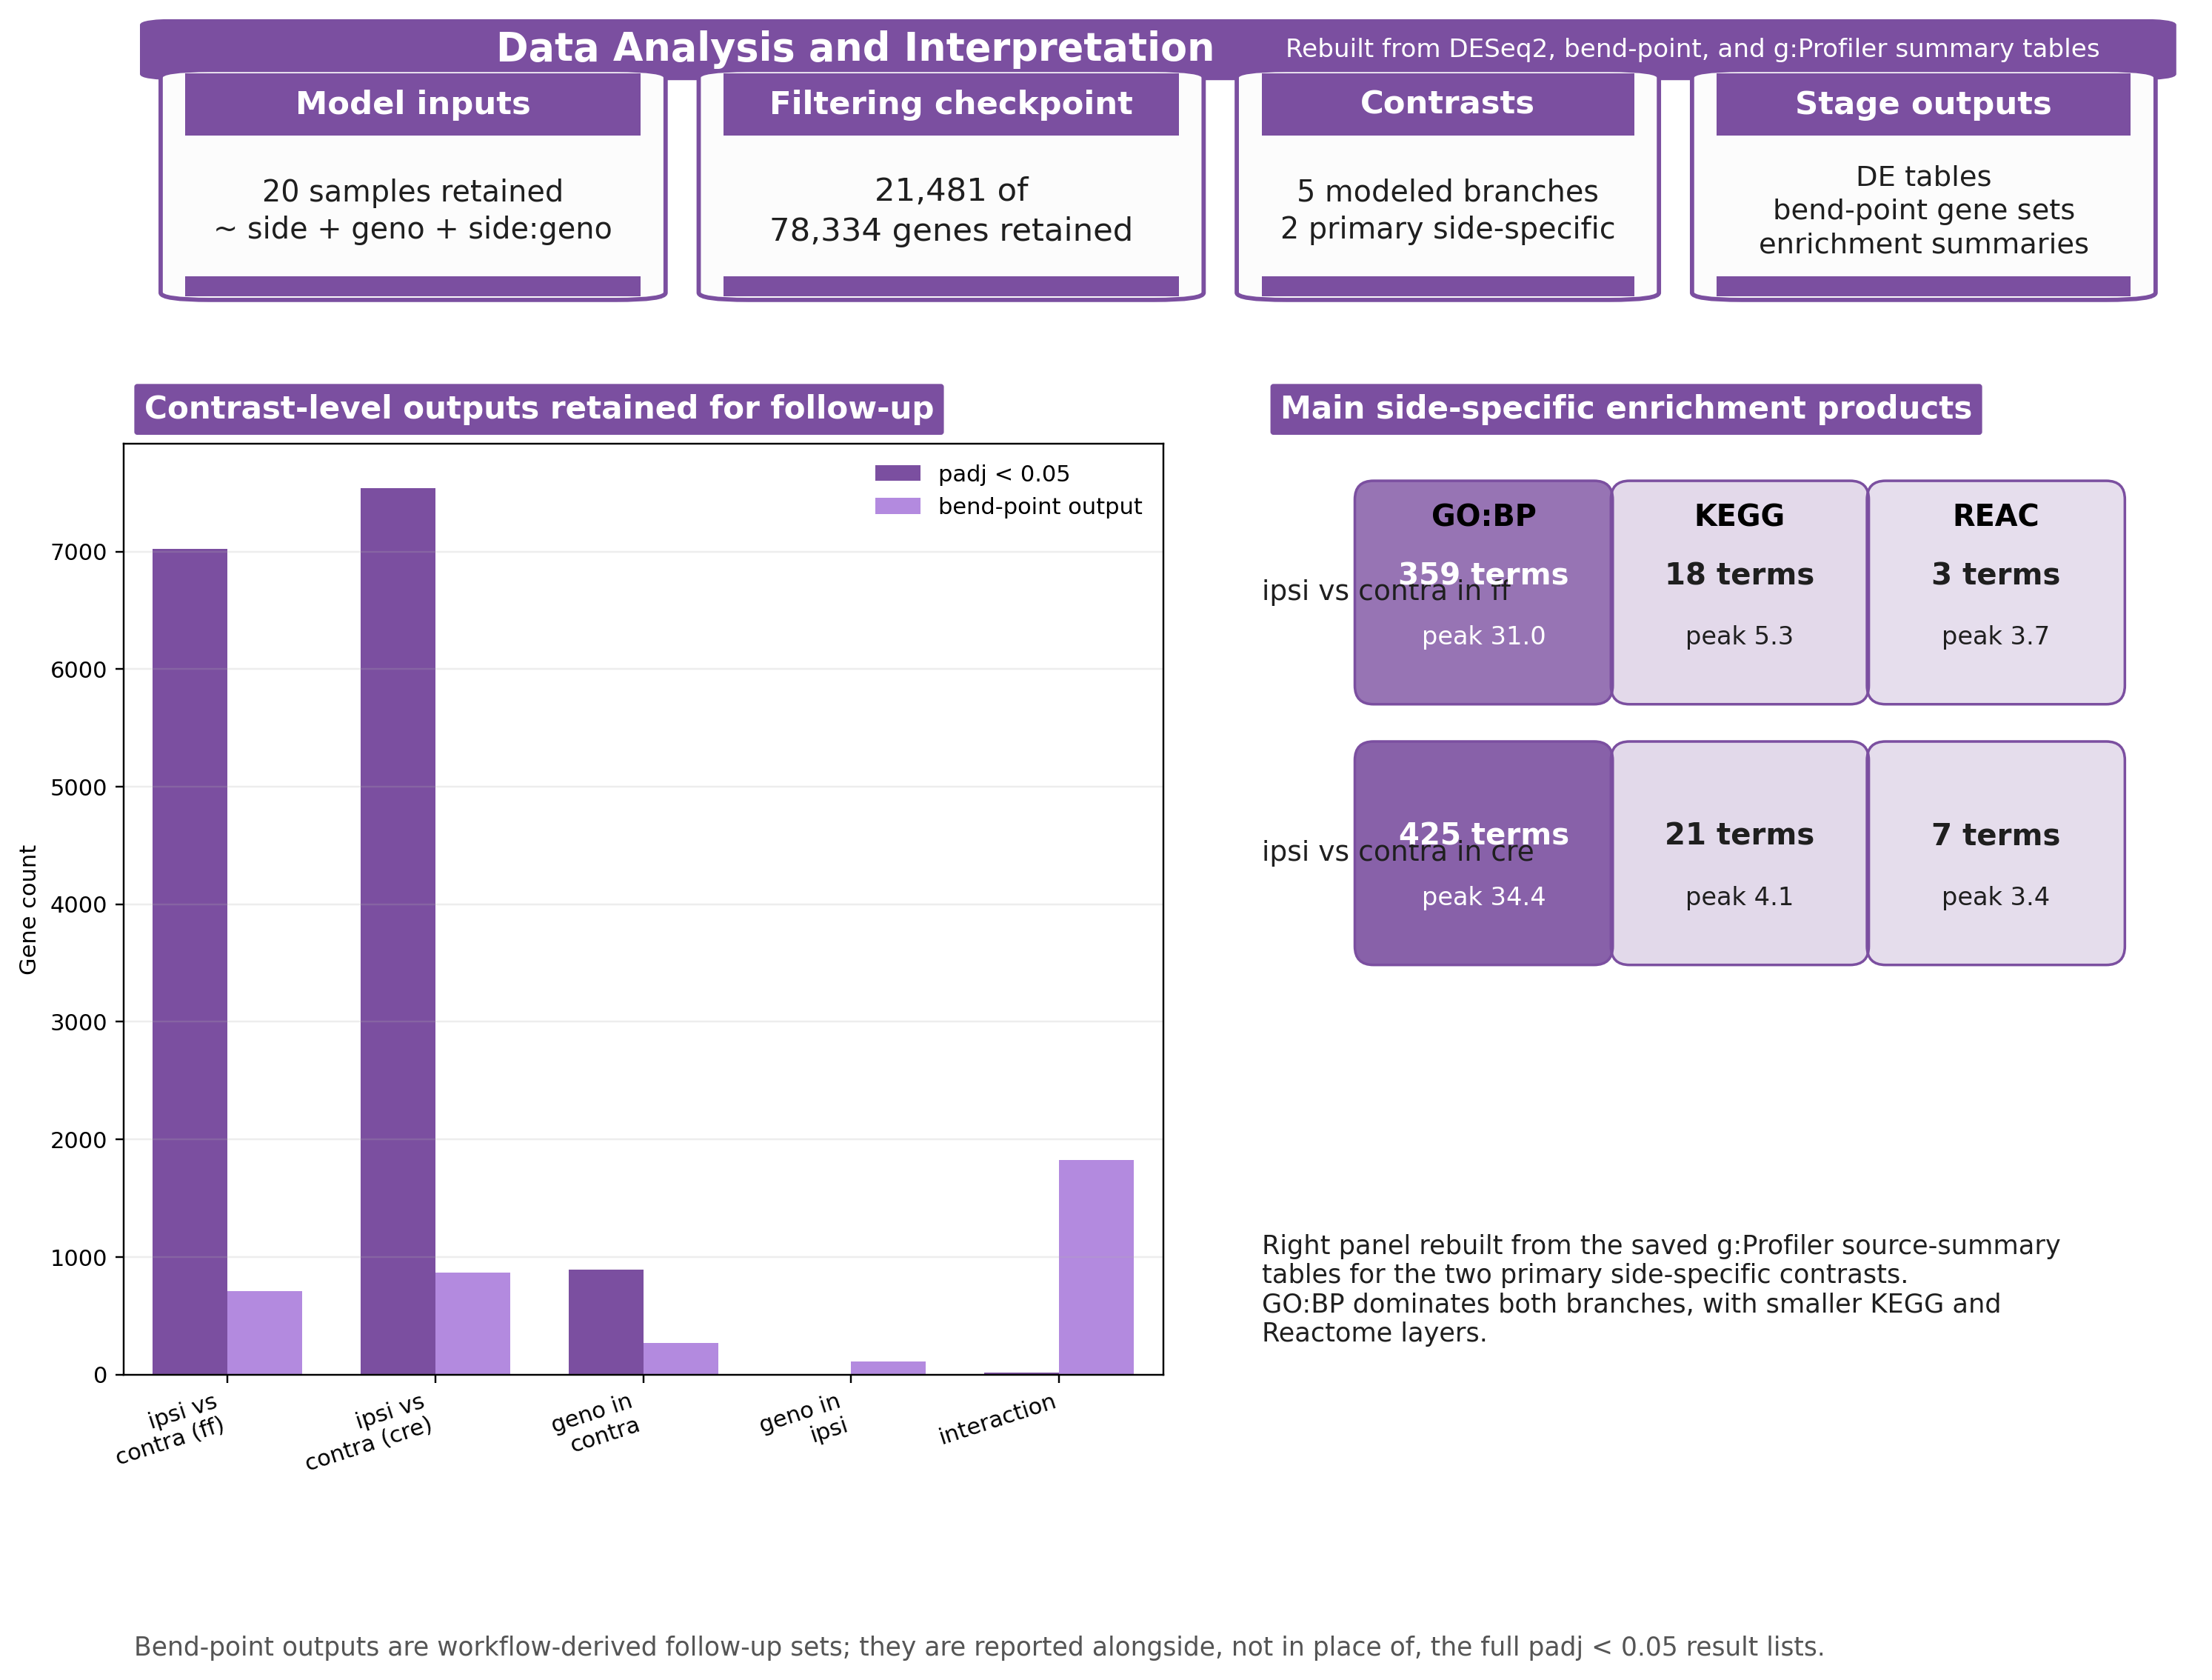
\includegraphics[width=\textwidth]{assets_methods/data_mining_stage.png}
\caption{Data Mining and Interpretation stage summary derived from the saved \texttt{DESeq2},
  bend-point, and enrichment outputs.
  Panel~(a): VST PCA showing the dominant \texttt{side\_class} separation on PC1 and the
  secondary genotype structure, with annotated FF/CRE pair distances.
  Panel~(b): ordered \textit{p}-value and cumulative-fraction curves for the primary
  \texttt{ipsi\_vs\_contra\_in\_ff} contrast, with the bend-point threshold
  ($1.37 \times 10^{-17}$; 709 genes) marked.
  Panel~(c): \texttt{g:Profiler} enrichment source summary for the same contrast
  (359~GO:BP, 18~KEGG, 3~Reactome terms).
  Volcano plots, MA plots, and heatmaps for all five contrasts are reserved for the
  Results section.}
\label{fig:data_mining}
\end{figure}


Across the section, the design principle was to let figures explain \emph{how} each pipeline
stage was executed and let tables capture \emph{what} each stage produced.
Color coding is applied at two levels: stage identity (blue / teal / amber / purple for
Collection, Cleaning, Preparation, and Mining) and, within the Mining stage, contrast priority
(deeper purple for primary contrasts, mid-purple for supporting genotype contrasts, and pale
purple for the contextual interaction contrast).
This layered coding makes the status of each analytical product visible at a glance without
requiring additional legend text in the narrative.


\end{document}
